\chapter{Subdivison Tools und Bibliotheken}

Im Bereich Subdivison Algorithmen gibt es schon viele mächtige Bibliotheken und Datenstrukturen.
Für das Team-Projekt bietet es sich an, diese zu evaluieren und passende Basisfunktionen wiederzuverwenden.
Dieses Kapitel vergleicht die gängigen C++-Bibliotheken und Datenstrukturen. Für


\section{OpenMesh}

OpenMesh wird von der \acs{RWTH} Aachen entwickelt und stellt eine mächtige Datenstruktur für polygonale Netze bereit.
Es steht unter der \acs{LGPL} v3 Lizenz ("with exception") und kann für unseren Fall somit problemlos verwendet werden.

\subsection{Datenstrukturen und Algorithmen}

OpenMesh implementiert eine Datenstruktur für polygonale Meshes. Darüber hinaus sind sogar bereits einige Subdivision Algorithmen implementiert, die auf der OpenMesh Datenstruktur arbeiten können. Zum Funktionsumfang gehören folgende Algorithmen.
\begin{enumerate}
\item Uniform subdivision
\begin{itemize}
	\item Loop
	\item SQRT3
	\item Modified Butterfly
	\item Interpolationg SQRT3 LG
	\item Composite
	\item Catmull Clark
\end{itemize}
\item Adaptive subdivision
\begin{itemize}
	\item Adaptive Composite
\end{itemize}
\item Simple subdivision
\begin{itemize}
	\item Longest Edge
\end{itemize}
\end{enumerate}

OpenMesh implementiert eine \emph{halfedge} Datenstruktur.
Diese \emph{edge-based} Datenstrukturen speichern die Information über die Verbindungen zwischen Eckpunkten (Vertices) in den Kanten (Edges), während
\emph{face-based} Datenstrukturen die Verbindungsinformation zwischen den Eckpunkten und Nachbarn in den Flächen (Face) speichern.\\
Jede Kante (Edge) referenziert also folgende Objekte:
\begin{itemize}
	\item 2 Eckpunkte (Vertices)
	\item eine Fläche (Face)
	\item die nächsten zwei Kanten (Edges) der Fläche
\end{itemize}

Halfedge bedeutet nun, dass eine Kante in 2 Halbkanten (Halfedge) aufgeteilt wird. Jede Halbkante hat nur eine Richtung.
Zwei Ecken A und B sind nun also über 2 Halbkanten (1. Halkante von A nach B und 2. Halbkante con B nach A) miteinander verbunden.
Dies bringt den Vorteil, dass man über die Kanten einer Fläche sehr einfach iterieren kann, man muss dazu lediglich den Halbkanten folgen.

\subsection{OpenFlipper}

Aufbauend auf OpenMesh wurde das flexible pluginbasierte Framework OpenFlipper enwickelt.
Damit können geometrische Objekte modelliert und verarbeitet werden können. Intern wird auf die Datenstrukur OpenMesh zurückgegriffen.
Für die grafische Oberfläche wird QT verwendet.
Mit OpenFlipper kann man über die Oberfläche einfache Netze erstellen und auch die in OpenMesh implementierten Subdivision Algorithmen anwenden.
Abbildung~\ref{fig:openflipper} zeigt die Benutzeroberfläche von OpenFlipper
\begin{figure}[h]
  \caption{OpenFlipper}
  \centering
  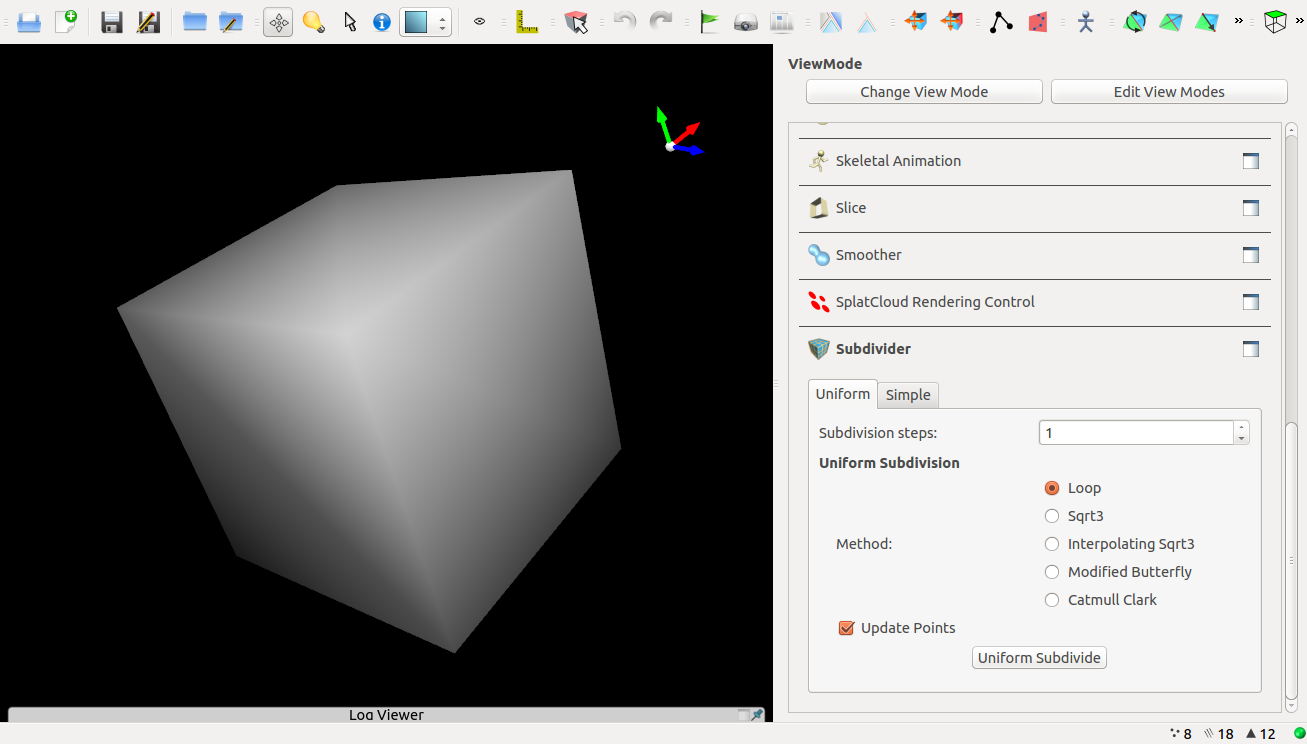
\includegraphics[width=0.8\textwidth]{content/media/openflipper_cube}
  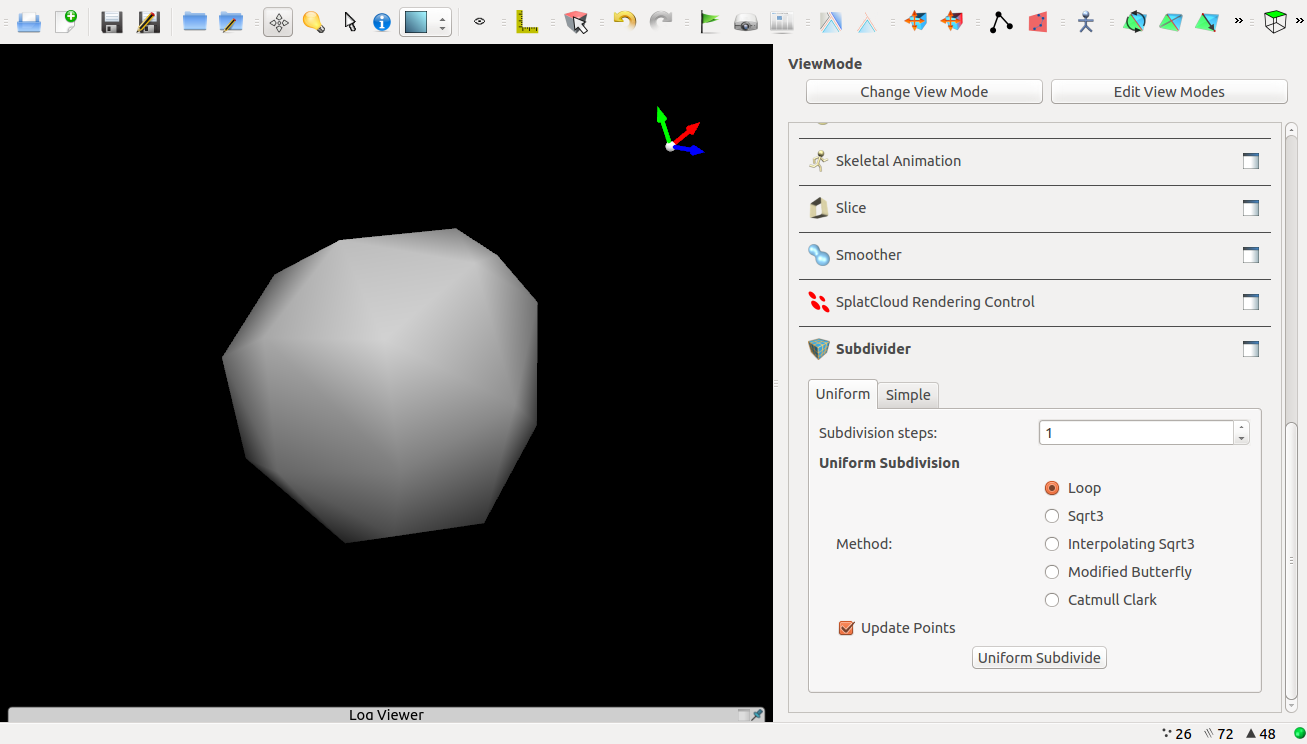
\includegraphics[width=0.8\textwidth]{content/media/openflipper_loop}
  \label{fig:openflipper}
\end{figure}


\section{Surface Mesh}

Surface Mesh ist eine einfache und effizente Datenstruktur um polygonale Netze beschreiben zu können.
Die Datenstruktur ist im Vergleich zu OpenMesh einfacher und implementiert nur die nötigsten Basisfunktionen.

// TODO

\section{OpenSubdiv}

Bibliothek für schnelles (<3ms) interaktives Rendering von Gitternetzen. Dabei wird mittel paralleler GPU-Berechnung gearbeitet und die Daten intern zwecks Optimierung umgewandelt. Leider wird momentan nur Catmull-Clark unterstützt. Für unsere Zwecke eher nicht geeignet.

// TODO


\section{CGoGN}

// TODO


\section{\acf{CGAL}}

// TODO


\section{Sonstige Tools}


\subsection{BViewer}

